\chapter{Methodology}
\label{chp:methodology}

\par This chapter discusses the methodology used to measure the effectiveness of \ac{ARG} at correctly classifying valid and invalid traffic, the shortest supportable hop interval at various network latencies, the maximum packet rate \ac{ARG} can handle, and the overall stability of the system under test. Section \ref{sec:problem_def} discusses the problem this research seeks to answer. Section \ref{sec:boundaries} defines the \ac{SUT}, and Section \ref{sec:services} goes into detail on the possible outcomes of the \ac{CUT}. Section \ref{sec:workload} covers the workload presented to the \ac{SUT}, Section \ref{sec:parameters} covers the configurable parameters of the \ac{SUT}, and Section \ref{sec:metrics} covers the metrics collected. Sections \ref{sec:eval_technique} and \ref{sec:exp_design} detail the actual tests and the purpose of each.

\section{Problem Definition}
\label{sec:problem_def}
\subsection{Goals and Hypothesis}
\label{sec:goals}
\par This research tests whether network address space randomization as discussed in Chapter \ref{chp:implementation} is suitable for deployment on a corporate or military network. Tests against this system are designed to answer four basic questions:

\begin{enumerate}
\item Does \ac{ARG} classify traffic correctly? What percentage of false positives (valid packets blocked) and false negatives (invalid traffic allowed through) does it introduce?
\item What is the maximum packet rate and throughput \ac{ARG} can support?
\item What is the minimum supportable time between hops? How does latency affect this?
\item Is \ac{ARG} stable when presented with corrupt, malformed, or replayed packets?
\end{enumerate}

%\par The software developed and tested here attempts to interfere minimally with the network, a critical requirement for the real-world deployment of such technology. Systems \ac{ARG} touches---both inside and outside the ``protected'' networks---do not need any modifications to continue to function. The research done here provides data on whether this is true as a side effect, potentially valuable information for an organization considering employing a \ac{DYNAT} solution. However, validation of this design goal is not a primary objective. 

%\par The working hypothesis for this research is, as speculated by Sandia, a \ac{DYNAT} system allows for quick identification of unexpected (and potentially malicious) packets entering a network. There are few identifiers within the scope of \ac{DYNAT} by which outgoing packets could be filtered. Given that, no filtering is done for outbound packets and hence no change in behavior is observed when compared to the control network. 

\par It is hypothesized that \ac{ARG} correctly classifies 99\% of traffic it encounters when operating with a hop interval appropriate for the network latency. In addition, this thesis hypothesizes that packet loss becomes acceptable when the hop interval matches or exceeds the one-way network latency, where acceptable loss is defined as less than 2\%. This percentage is based on the loss seen on Massachusetts Institute of Technology's wireless networks \cite{MITWifiLoss}. The other two questions are informational as the results apply only to this specific hopping gateway implementation, but it is believed that \ac{ARG} is stable in the face of malformed traffic and it can handle at least 10 \ac{Mbps} of traffic. 

\subsection{Approach}
\label{sec:approach}
\par This research is accomplished on a test network with nodes representing the types of hosts found on a typical, corporate-style network. These include trusted hosts inside trusted networks which communicate freely, internal and external servers that must be accessible to hosts inside these trusted networks, and malicious hosts outside the networks. A configurable custom hopping gateway sits in front of the trusted networks. 

\par Traffic generators and collectors run on the test network, determining which traffic flows successfully make it to their intended destination. This includes examining both false positive and false negative rates, determining why \ac{ARG} rejects packets that should get through and why it allows packets that should be rejected. After a given test, logs and traffic captures are collated to form a complete picture of the traffic on the network before determining statistics.

\section{System Boundaries}
\label{sec:boundaries}
\par The \ac{SUT} is \ac{ARG}, the custom \ac{IP} hopping gateway developed specifically for this effort. The basic components of this system, the various inputs into the system, possible outputs, and the metrics provided are illustrated in Figure \ref{fig:sut}. The sections following cover aspects of this diagram in more detail, with Section \ref{sec:services} discussing the possible outcomes, Section \ref{sec:workload} covering the workload, Section \ref{sec:parameters} detailing the parameters in use, and Section \ref{sec:metrics} covering the metrics collected.

\begin{figure}
\caption{\ac{ARG} \ac{SUT} diagram}
\label{fig:sut}
\centering
\noindent\makebox[\textwidth]{%
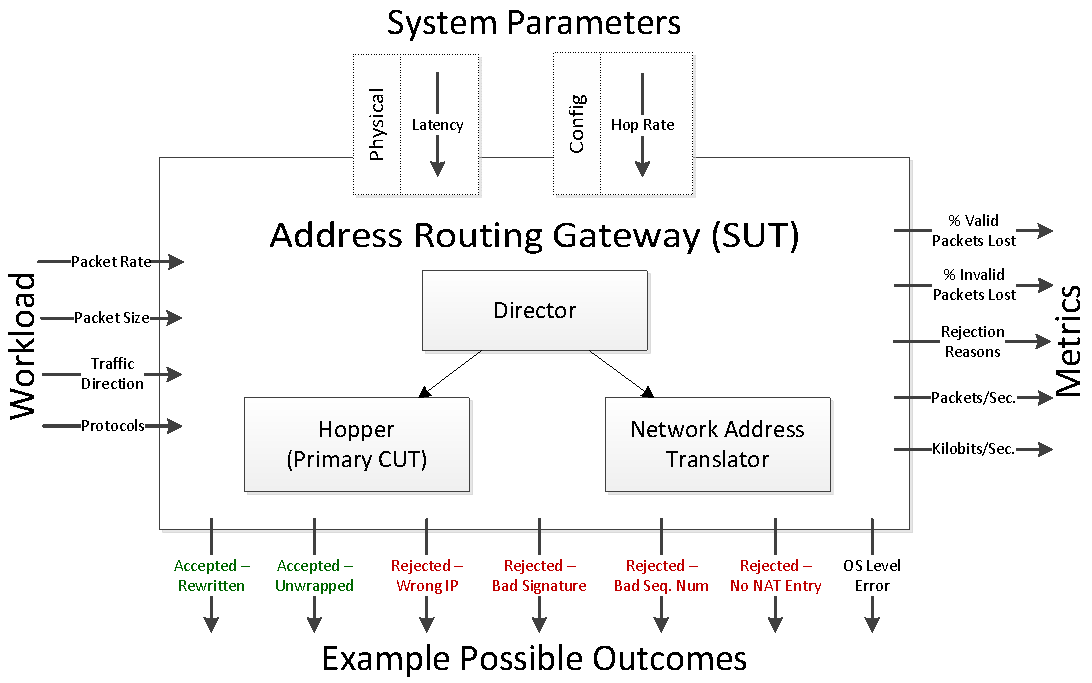
\includegraphics[width=1.22\textwidth]{sut}
}
\end{figure}

\section{System Services}
\label{sec:services}
\par This thesis tests three components of \ac{ARG}. Most important is the hopper module, which provides a rapidly-changing external \ac{IP} address and details on connected ARG networks. Using this information, it transports packets between ARG-protected networks. Packets to and from external hosts---hosts that are not part of an ARG network---go through the \ac{NAT} module. Finally, the director module hands packets off to each of the other modules and collects the results back to be logged and potentially acted upon. More details on these components are in Chapter \ref{chp:implementation}.

\par The potential outcomes of the director are shown below, broken into separate sections based on incoming or outgoing packets. Other services do not directly offer outcomes relevant to this research.

\begin{itemize}
\item Director - Incoming
	\begin{itemize}
	\item Accepted: Rewritten and forwarded - Packet is from non-\ac{ARG} network and is rewritten via \ac{NAT} table before forwarding.
	\item Accepted: Unwrapped and forwarded - Packet is from \ac{ARG} network and passes validation checks. Contents are extracted and forwarded internally.

	\item Rejected: Incorrect source \ac{IP} - Packet is coming from an \ac{ARG} network but does not have what the local gateway believes is the current source IP for the other gateway.
	\item Rejected: Incorrect destination \ac{IP} - Packet is coming from an \ac{ARG} network but does not have the current local gateway \ac{IP} as the destination.
	\item Rejected: Incorrect message size - The message length does not match the message type.
	\item Rejected: Incorrect sequence number - The message's sequence number is not monotonically increasing. 
	\item Rejected: Unable to verify signature/\ac{HMAC} - Packet signature invalid/nonexistent (if coming from an \ac{ARG} network).
	\item Rejected: No \ac{NAT} bucket/entry - Packet is coming from a non-\ac{ARG} network but does not have a valid entry in the \ac{NAT} table.

	\item Rejected: Misc - Some operating system-level errors may occur, resulting in rare errors in sending or receiving packets.
	\end{itemize}

\newpage
\item Director - Outgoing
	\begin{itemize}
	\item Accepted: Rewritten and forwarded - Packet is destined for non-\ac{ARG} network. An entry is made/retrieved from the \ac{NAT} table and used to rewrite packet.

	\item Rejected: Gateway not connected - Packet was intended for an ARG network the gateway is aware of but not yet connected to.
	\item Rejected: Wrapped and forwarded - Packet is destined for an \ac{ARG} network. Wrapped and placed on the external network.

	\item Rejected: Misc - Some operating system-level errors may occur, resulting in rare errors in sending or receiving packets.
	\end{itemize}
\end{itemize}

\section{Workload}
\label{sec:workload}
\par Workload to the system is the traffic flowing through the \ac{ARG} gateways. Standard network traffic parameters like packet rate, packet size, protocol types, number of simultaneous ongoing connections, and lifetime of connections play a role. For the purposes of this thesis, however, packet rate is the primary factor. Each test involves traffic generators, all of which may be instructed to wait a given amount of time between each sent packet. The lower the packet delay, the higher the packet rate.

\par It is important to note that network performance itself is not a large concern of this research. Packet rate does provide useful information about the performance of \ac{ARG}, but the numbers apply only to this specific implementation. \ac{ARG}'s development does not focus on performance in this first iteration, leaving many possible areas for improvement. Previous research has shown that similar solutions have minimal impact on performance \cite{NAH}. 

\par All traffic generators in the tests create randomly-sized packets of either \ac{UDP} or \ac{TCP} traffic. The protocol used depends on the test being run at the time; Section \ref{sec:exp_design} discusses each test series and the traffic flows they utilize.

\section{System Parameters}
\label{sec:parameters}
\par As a network application, \ac{ARG} is affected by both the machine on which it runs and the network over which it communicates. \ac{ARG}'s local performance is most affected by processor and memory speeds, with encryption potentially consuming a fair amount of processor time and memory speeds impacting virtually all aspects of operation.

\par The primary physical network parameter that affects \ac{ARG} is latency. To ensure that two \ac{ARG} gateways are able to communicate reliably, packets sent from one gateway to the other must arrive before the \ac{IP} addresses used in the send are no longer current. If hops occur too frequently, a high one-way latency will cause sent packets to frequently arrive after the receiving gateway has hopped to a different \ac{IP} address. (Adapting to latency is an area of potential improvement, as Section \ref{sec:future_work} discusses.) The test environment inherently introduces less than one millisecond of latency, but artificial latency can be added to simulate a more realistic range of network conditions.

\par The primary configuration setting for \ac{ARG} is the hop interval. \ac{ARG} allows the time between hops to be customized from several times a second to minutes apart with millisecond precision. Each gateway may be configured to hop at different rates, but for the sake of this thesis the hop intervals for each gateway are identical in a given test. 

\section{Evaluation Technique}
\label{sec:eval_technique}
\par Measurement is used to obtain results for each factor level. Due to the fairly complex interactions needed between \ac{ARG} gateways and the processing needed to decide how to handle packets, simulating the system would likely require an equal amount of work with little benefit.

\par Setup of the test environment involves a basic seven-node network: three gateways running \ac{ARG}, one system on the network protected by each gateway, and one host outside the network. Figure \ref{fig:argnetwork} shows the network and the names given to the various systems.

\begin{figure}
	\centering
	\caption{\ac{ARG} test network layout overview}
	\label{fig:argnetwork}
	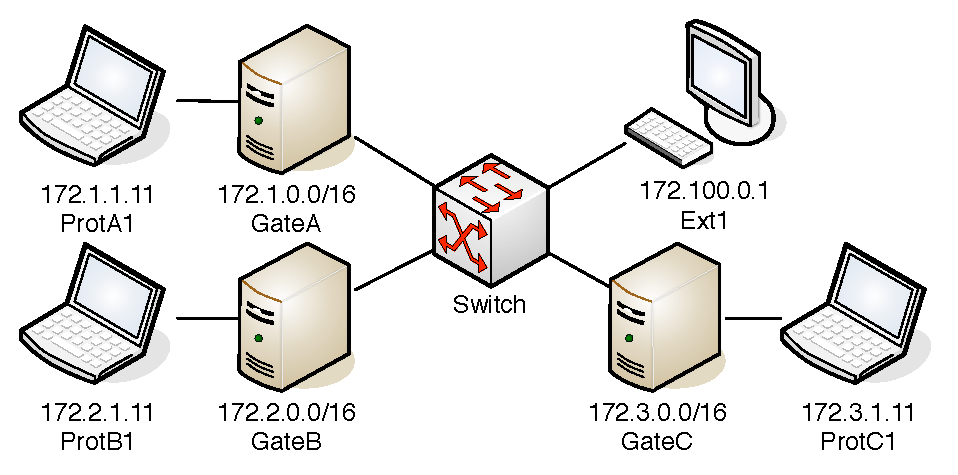
\includegraphics[width=0.75\textwidth]{thesis_network}
\end{figure}

\par Protected clients behind the gateways (\texttt{ProtA1}, \texttt{ProtB1}, and \texttt{ProtC1}) may communicate freely. The protected clients may also talk out to the external host (\texttt{Ext1}), and the external hosts must then---once that connection is established---be able to talk back into the network. There is additional administrative traffic directly between the gateways (\texttt{GateA}, \texttt{GateB}, and \texttt{GateC}). These three basic traffic flows are ``valid'' traffic.

\par All traffic beyond what is described above is ``invalid.'' For example, \texttt{Ext1} is not allowed to send traffic in to the protected clients or the gateways without them first initiating the connection. Malformed traffic sent by any host is also considered invalid. In either case, invalid traffic should be stopped at the earliest possible opportunity (i.e., the gateway rejects the packet and keeps it from reaching the internal host) and the gateway must remain stable.

\par To collect data, each system runs the traffic collection program \texttt{tcpdump} to capture traffic sent and received into \ac{PCAP} files. The test execution script then spawns traffic generators on the correct systems in the network, based on what test is being run. Section \ref{sec:exp_design} details the types of traffic each test establishes. Each traffic generator logs their sends and receives to text log files (one per generator), independent of the \texttt{tcpdump} traffic captures. After a given trial, the \ac{PCAP} files and traffic generator logs are collated and processed with custom scripts to determine the metrics described in Section \ref{sec:metrics}. More details on the traffic generators and test run sequence can be found in Appendixes \ref{chp:testseq} and \ref{chp:generators}. Appendix \ref{chp:processor} covers the custom results processor.

\par All trials run on a network of seven physical servers. Each server runs Ubuntu 12.04.1 Server Edition with four gigabytes of \ac{RAM} and a 2.6 gigahertz quad-core Intel Xeon. A single switch with four \acp{VLAN} connects each system at 100 \ac{Mbps}.

\section{Performance Metrics}
\label{sec:metrics}
\par As previously stated, this research primarily focuses on the classification accuracy of \ac{ARG} and the interaction of the hop interval and latency. Measurements on \ac{ARG} therefore concentrate on the outcomes from the director. However, basic statistics on network performance are collected. The metrics of interest include:

\begin{itemize}
\item Percentage of invalid packets accepted
	\par If a packet that should have been rejected is accepted by \ac{ARG}, it is possible for an attacker to sneak into the network regardless of the gateway's existence. This is the true measure of whether or not \ac{ARG} is protecting the network. If \ac{ARG} functions correctly, this number should remain at zero for all experiments with \ac{ARG} enabled.

\item Percentage of valid packets rejected
	\par In ideal circumstances, this will also be zero. However, network conditions may result in failures here, which on a real-world network might result in a disruption of service. 

\item Number of each type of rejection (each possible outcome from the director)
	\par This reveals where in the processing stage packets are typically caught. If packets get caught in the later stages of validation---e.g., signature checking---then processing time has been wasted.

\item Packets per second and \acf{Kbps}
	\par An easy check on \ac{ARG}'s performance is comparing the amount of traffic it is handling against the packet loss it shows. Information about both the number of packets and the raw number of bits it processes may reveal slightly different results, so both are collected.
\end{itemize}

\section{Experimental Design}
\label{sec:exp_design}
\par Based on the system and workload parameters given in Sections \ref{sec:workload} and \ref{sec:parameters} and the goals of this research (as presented in Section \ref{sec:goals}), there are eight traffic flows of interest. Each consists of different types of traffic and flow destinations. These are most easily visualized in Figure \ref{fig:testnum_flows} on page \pageref{fig:testnum_flows}.

\begin{figure}
\caption[Experiment traffic flow directions and protocols]{Experiment traffic flow directions and protocols. Black solid lines indicate valid traffic, red dashed lines are invalid.}
\label{fig:testnum_flows}
\centering
\begin{subfigure}[b]{0.328\linewidth}
	\centering
	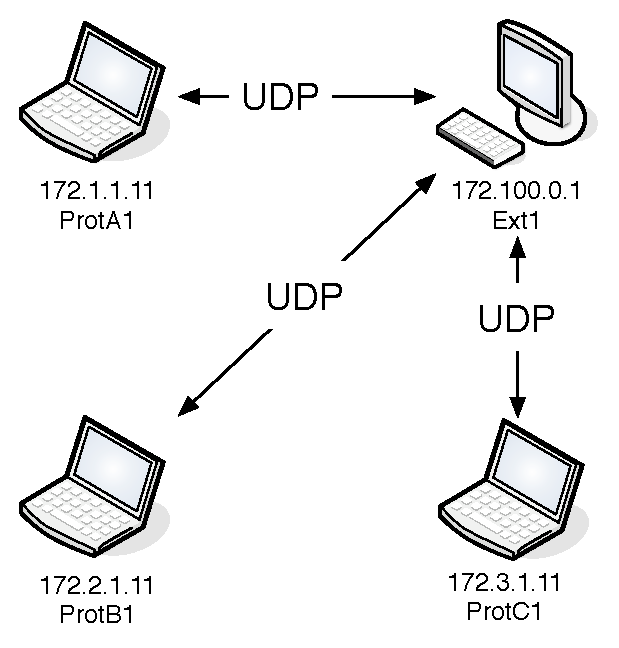
\includegraphics[width=1.0\linewidth]{test_traffic_0}
	\caption{Flow 0}
\end{subfigure}
\begin{subfigure}[b]{0.328\linewidth}
	\centering
	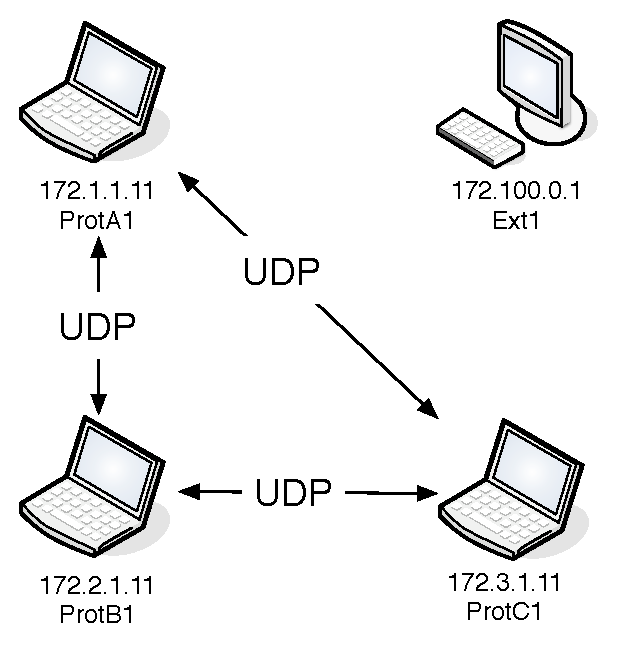
\includegraphics[width=1.0\linewidth]{test_traffic_1}
	\caption{Flow 1}
\end{subfigure}
\begin{subfigure}[b]{0.328\linewidth}
	\centering
	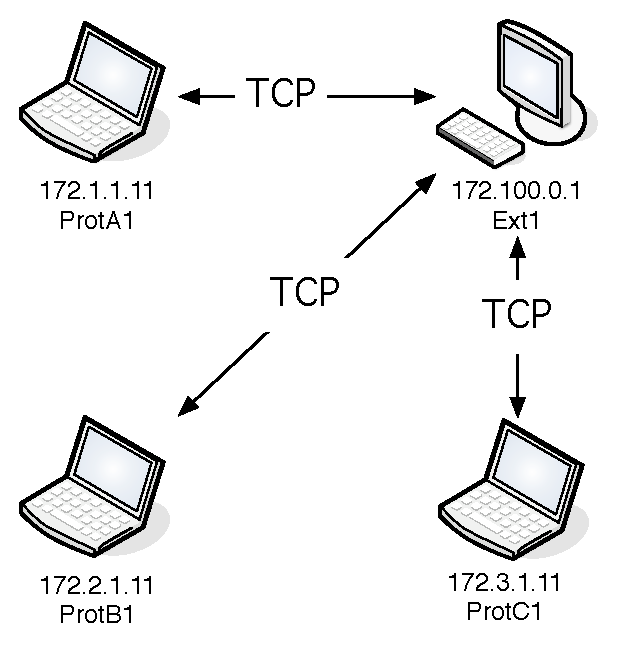
\includegraphics[width=1.0\linewidth]{test_traffic_2}
	\caption{Flow 2}
\end{subfigure}
\begin{subfigure}[b]{0.328\linewidth}
	\centering
	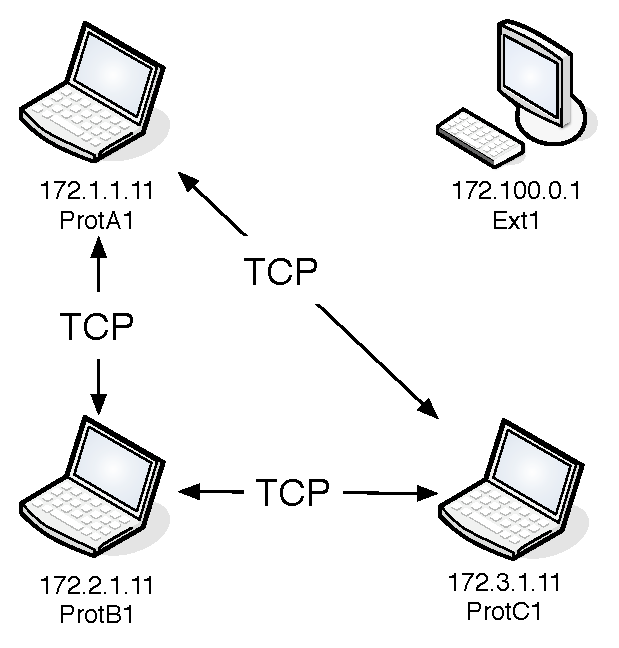
\includegraphics[width=1.0\linewidth]{test_traffic_3}
	\caption{Flow 3}
\end{subfigure}
\begin{subfigure}[b]{0.328\linewidth}
	\centering
	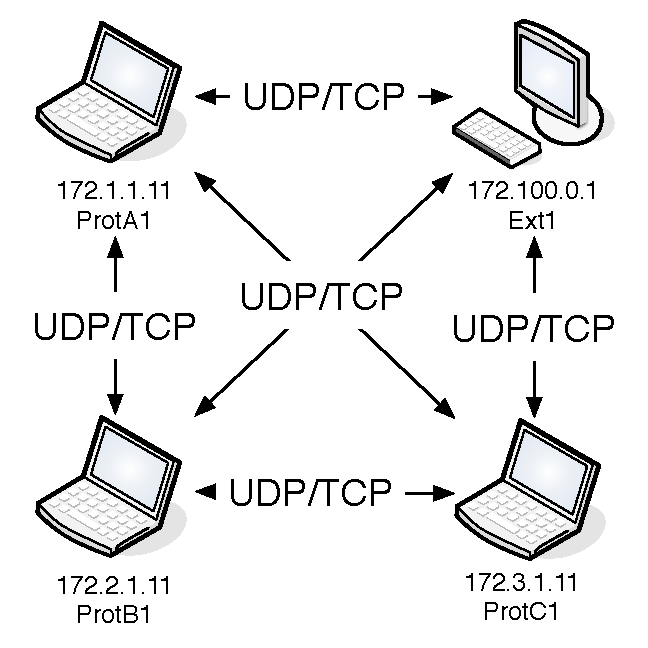
\includegraphics[width=1.0\linewidth]{test_traffic_4}
	\caption{Flow 4}
\end{subfigure}
\begin{subfigure}[b]{0.328\linewidth}
	\centering
	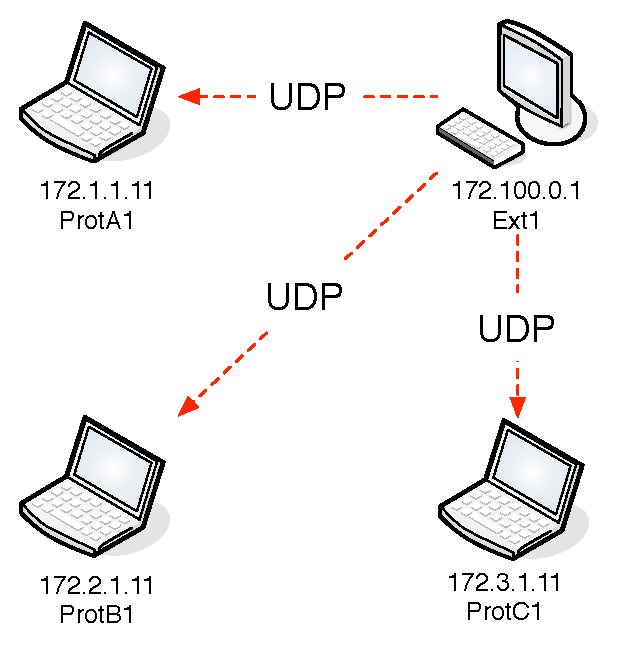
\includegraphics[width=1.0\linewidth]{test_traffic_5}
	\caption{Flow 5}
\end{subfigure}
\begin{subfigure}[b]{0.328\linewidth}
	\centering
	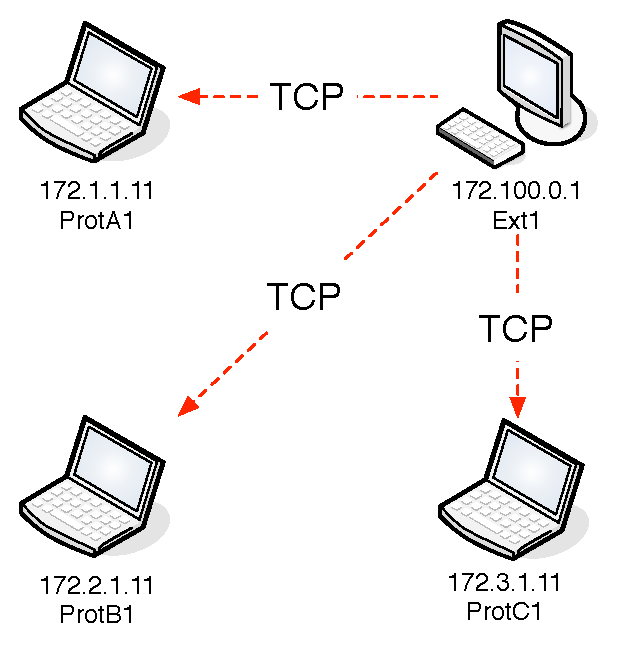
\includegraphics[width=1.0\linewidth]{test_traffic_6}
	\caption{Flow 6}
\end{subfigure}
\begin{subfigure}[b]{0.328\linewidth}
	\centering
	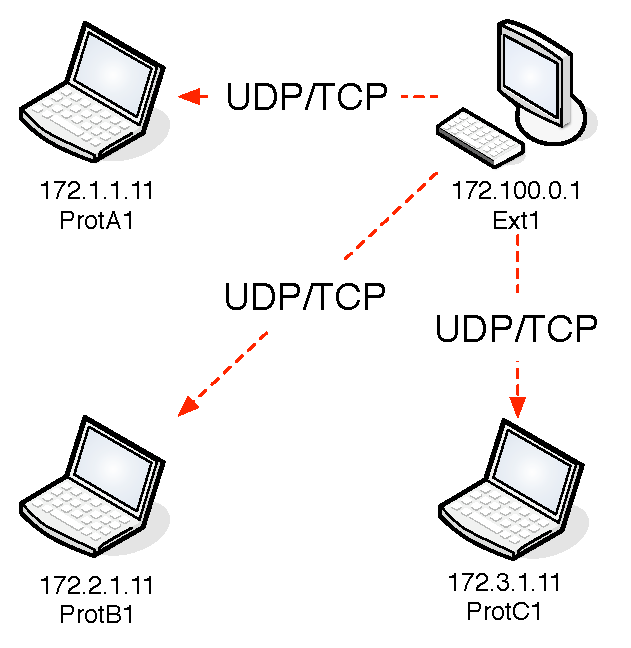
\includegraphics[width=1.0\linewidth]{test_traffic_7}
	\caption{Flow 7}
\end{subfigure}
\begin{subfigure}[b]{0.328\linewidth}
	\centering
	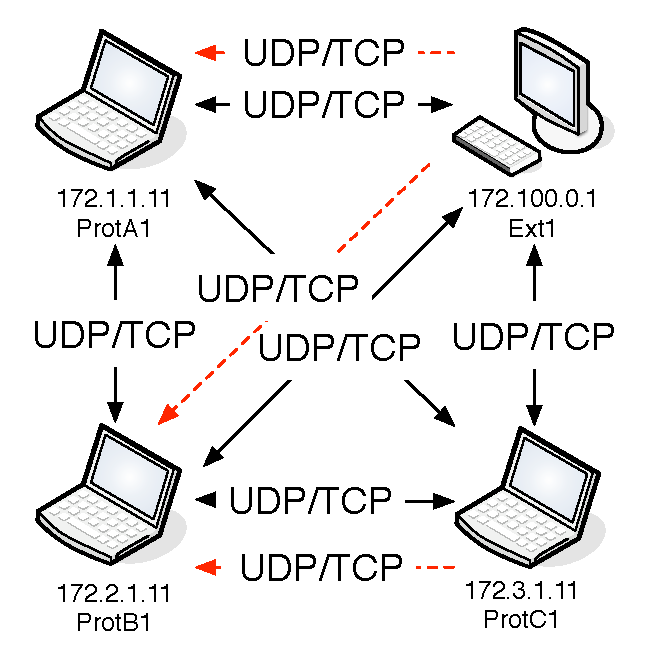
\includegraphics[width=1.0\linewidth]{test_traffic_8}
	\caption{Flow 8}
\end{subfigure}
\end{figure}

\par These possible traffic flows are used in four sets of experiments, given below. Each experiment set answers a different research goal and utilizes different factor levels, as shown in their respective tables.

\begin{itemize}
	\item Basic tests
	\par Table \ref{tbl:basic_factors} displays the factor levels used for this series of tests. This sequence of tests verifies that \ac{ARG} classifies traffic correctly by running every test shown in Figure \ref{fig:testnum_flows} against \ac{ARG}. Latency is set to 20 milliseconds (\ac{RTT}) for all tests and traffic generators produce packets around every 0.3 seconds. To determine if the time between hops has a statistically significant impact on certain types of traffic, every test runs twice, once with a long hop interval of 500 milliseconds and once with a shorter interval of 50 milliseconds, which is just slightly more than double the round-trip latency.

\begin{table}
\caption{Factor levels for basic tests}
\label{tbl:basic_factors}
\centering
\begin{tabular}{ll}
\toprule
\textbf{Factor} & \textbf{Possible Levels} \\
\hline
Hop interval (ms) & 500, 50\\
Round-trip latency (ms) & 20\\
Packet delay (s) & 0.3\\
Traffic direction and type & Flows 0--8 (See Figure \ref{fig:testnum_flows})\\
\bottomrule
\end{tabular}
\end{table}

	\item Maximum Throughput
	\par Table \ref{tbl:throughput_factors} displays the factor levels used for this series of tests. This sequence gives an indication of what throughput and packet rate \ac{ARG} is capable of handling. Packet delay goes through all levels shown, which leads to roughly corresponding increases in the throughput the gateways must handle. As with the basic tests, the hop interval alternates between 500 ms and 50 ms to see if the additional \ac{IP} calculation load impacts the maximum rate. Flow 4 is used across all runs to because it utilizes both \ac{TCP} and \ac{UDP} traffic flowing in all valid directions. \ac{RTT} is set to 20 ms.

\begin{table}
\caption{Factor levels for throughput tests}
\label{tbl:throughput_factors}
\centering
\begin{tabular}{ll}
\toprule
\textbf{Factor} & \textbf{Possible Levels} \\
\hline
Hop interval (ms) & 500, 50\\
Round-trip latency (ms) & 20\\
Packet delay (s) & 0.2, 0.1, 0.05, 0.01, 0.005, 0.001\\
Traffic direction and type & Flow 4 (See Figure \ref{fig:testnum_flows})\\
\bottomrule
\end{tabular}
\end{table}

	\item Minimum hop interval 
	\par Table \ref{tbl:hoprate_factors} displays the factor levels used for this series of tests. This sequence determines the minimum time between \ac{IP} address changes at various latencies. The hop interval and latency go through the levels shown in a full factorial fashion (every latency-hop interval combination). Packet rate is fixed at 0.3 seconds. Flow 4 is used throughout.

\begin{table}
\caption{Factor levels for minimum hop interval tests}
\label{tbl:hoprate_factors}
\centering
\begin{tabular}{ll}
\toprule
\textbf{Factor} & \textbf{Possible Levels} \\
\hline
Hop interval (ms) & 1000, 500, 300, 200, 100, 75, 60, 50, 40, 30, 15, 10, 5\\
Round-trip latency (ms) & 0, 30, 100, 500\\
Packet delay (s) & 0.3\\
Traffic direction and type & Flow 4 (See Figure \ref{fig:testnum_flows})\\
\bottomrule
\end{tabular}
\end{table}

	\item Fuzzer
	\par Table \ref{tbl:fuzz_factors} displays the factor levels used for this series of tests. This sequence is not tested rigorously for traffic flow success and failure, but ensures that \ac{ARG} remains stable despite malformed traffic. Traffic Flow 8 is used, with additional traffic coming from fuzzers running that replay and/or alter all gateway traffic they see. Hop intervals vary between 500 ms and 50 ms, latency is fixed at 20 ms, and packets are sent at 0.3 second intervals.

\begin{table}
\caption{Factor levels for fuzz tests}
\label{tbl:fuzz_factors}
\centering
\begin{tabular}{ll}
\toprule
\textbf{Factor} & \textbf{Possible Levels} \\
\hline
Hop interval (ms) & 500, 50\\
Round-trip latency (ms) & 20\\
Packet delay (s) & 0.3\\
Traffic direction and type & Flow 8 (See Figure \ref{fig:testnum_flows})\\
\bottomrule
\end{tabular}
\end{table}
\end{itemize}

\par A 95\% confidence interval is used for all experiments. Experiments are each run for five minutes, sufficient time for the system to stabilize (pilot studies show that \ac{ARG} fully connects in under 10 seconds on the test network). Some variation is possible in the actual traffic seen in a single run, so a minimum of 10 replications are used for each experiment.

\section{Summary}
\label{sec:method_summary}
\par This chapter discusses the goals of this research and defines the \ac{SUT} and its relevant factors. The methodology in use is covered, with details on the test network and the exact tests run on this network. Finally, this chapter enumerates the metrics the tests collect and analyze. 

